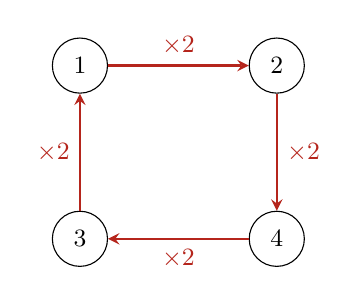
\begin{tikzpicture}[>=stealth,font=\small]
\foreach \x/\y/\v in {0/1.1/1,2.5/1.1/2,2.5/-1.1/4,0/-1.1/3}{\node[draw,circle,minimum size=.7cm] (n\v) at (\x,\y) {$\v$};}
\draw[->,BrickRed,thick] (n1)--node[above] {$\times2$}(n2);
\draw[->,BrickRed,thick] (n2)--node[right] {$\times2$}(n4);
\draw[->,BrickRed,thick] (n4)--node[below] {$\times2$}(n3);
\draw[->,BrickRed,thick] (n3)--node[left] {$\times2$}(n1);
\end{tikzpicture}
